\chapter{Analise do problema e desenho de uma solução}
\label{chap:analisedoproblema}

\textit{Adicionar texto introdutorio}

\section{O Dominio}

Este projeto teve como objetivo principal o desenvolvimento de uma plataforma ajustada às necessidades da organização e aos desafios por ela apresentados. Para tal, tornou-se essencial definir e estruturar cuidadosamente a lógica de negócio subjacente.

Após várias sessões de discussão com os professores envolvidos, foi possível clarificar o domínio do problema e estabelecer uma visão mais sólida sobre a solução pretendida. Ao longo dos meses, essa visão foi sendo progressivamente aperfeiçoada, permitindo alinhar melhor os requisitos com os objetivos do projeto.

\begin{figure}    
    \centering
    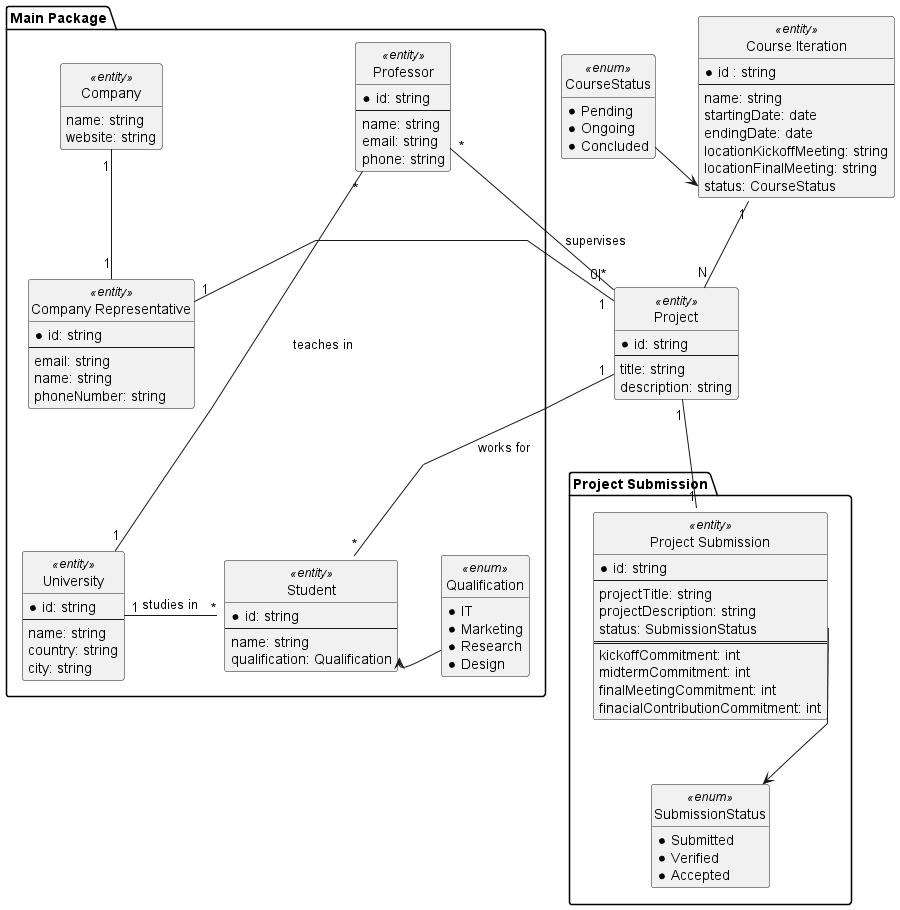
\includegraphics[width=\linewidth]{capitulos/cap3-analisedoproblema/assets/domain-diagram/dd.png}
    \caption{Diagrama de classes da lógica de negócio do Blended4Future 1}
    \label{fig:dd}
\end{figure}


A figura \ref{fig:dd} refere-se ao diagrama finalizado que foi definido.

\section{Engenharia de requisitos}

A Engenharia de Requisitos é uma área da Engenharia de Software que se dedica à identificação, análise, especificação, validação e gestão das necessidades e expectativas das partes interessadas relativamente a um sistema, com o objetivo de transformar essas necessidades, muitas vezes vagas ou incompletas, em requisitos claros, compreensíveis e verificáveis.

Esta secção dedica-se à apresentação dos requisitos estabelecidos para o sistema no arranque do projeto. 
Para uma melhor organização, estes requisitos foram divididos em dois grupos distintos: funcionais, que descrevem as operações fundamentais que a aplicação deve garantir, e não funcionais, que representam as condições e restrições que asseguram o correto desempenho dessas operações.


\subsection{Requisitos funcionais}
\label{subsection:requisitos_funcionais}

Durantes os primeiros dois sprints, em conjunto dos professores, foi estabelecido um \textit{backlog} de \textit{user stories} que refletia a experiência desejada dos atores. 

A tabela \ref{tab:req-funcionais} reflete esta decisão.
\subsubsection{Diagram de \textit{User Flow}}

Um Diagrama de \textit{User Flow} é uma representação visual que descreve o caminho que um utilizador percorre dentro de um sistema ou aplicação para atingir um objetivo específico. Para uma melhor experiência de desenvolvimento, um destes foi elaborado. Este pode ser encontrado no anexo \ref{app:userflowchart}.    

\subsection{Requisitos não Funcionais}

\subsubsection{FURPS}
Para organizar e clarificar os requisitos do sistema, recorreu-se ao modelo \textbf{FURPS}, que permite classificar os requisitos em cinco categorias: 

\paragraph{Functionality (Funcionalidade)}
\begin{itemize}
    \item Funcionalidades de backoffice e frontoffice asseguradas com a respetiva autenticação.
\end{itemize}

\paragraph{Usability (Usabilidade)}
\begin{itemize}
    \item Interface intuitiva e consistente, que siga as normas de design.
    \item Navegação simples, permitindo localizar facilmente projetos e conteúdos.
    \item Feedback visual claro sobre ações realizadas (erros, confirmações).
\end{itemize}

\paragraph{Reliability (Confiabilidade)}
\begin{itemize}
    \item Garantir que o programa se mantém ativo e disponivel, mesmo na presença de erros e outras adversidades.
    \item Assegurar que novas versões são disponibilizadas sem prejudicar a persistência de informação na base de dados.
\end{itemize}

\paragraph{Performance (Desempenho)}
\begin{itemize}
    \item Resposta rápida da interface mesmo com múltiplos utilizadores.
\end{itemize}

\paragraph{Supportability (Suportabilidade)}
\begin{itemize}
    \item Código modular e documentado para facilitar manutenção futura.
    \item Facilita a adição de novas funcionalidades ou integração com outras ferramentas.
\end{itemize}


Algumas destes requisitos foram considerados como casos de uso do programa e adicionados à tabela referida no ponto \ref{subsection:requisitos_funcionais} de forma a facilitar o processo de desenvolvimento. A tabela \ref{tab:req-nao-funcionais} subscreve esta decisão.

\begin{landscape}
\begin{longtable}{lp{20cm}}
\hline
    \textbf{User Story} & \textbf{Título} \\ \hline
    \endfirsthead

    \hline
    \textbf{User Story} & \textbf{Título} \\ \hline
    \endhead

    US2 & Como Representante da Empresa, quero alterar facilmente os detalhes da minha empresa (logótipo, contactos, etc.) para que represente melhor a sua imagem \\ \hline
    US3 & Como Representante da Empresa, quero submeter facilmente um novo projeto \\ \hline
    US4 & Como Empresa, quero relatórios com os resultados dos meus projetos. \\ \hline
    US6 & Como Professor, quero poder aceitar novas ideias de projeto \\ \hline
    US7 & Como Professor, quero poder selecionar um estudante e ver mais detalhes sobre ele (área de especialização, experiência profissional, LinkedIn) \\ \hline
    US8 & Como Professor, quero enviar convites a estudantes para participarem em projetos de acordo com as suas qualificações e interesses \\ \hline
    US9 & Como Estudante, gostaria de saber quais as qualificações necessárias para me inscrever num projeto \\ \hline
    US11 & Como Representante da Universidade, gostaria de poder contactar a Blended para aderir ao programa \\ \hline
    US12 & Como Utilizador, quero poder pesquisar projetos com base em critérios específicos \\ \hline
    US13 & Como Utilizador, quero receber uma confirmação por email após o registo para saber que a minha conta foi criada com sucesso \\ \hline
    US14 & Como Utilizador, quero ver uma página inicial \\ \hline
    US15 & Como Utilizador, gostaria de iniciar sessão na minha conta, para poder aceder às minhas informações pessoais \\ \hline
    US17 & Como Administrador, quero adicionar novas empresas ao sistema com o respetivo site e logótipo, para que a sua parceria seja visível na plataforma \\ \hline
    US18 & Como Administrador, quero poder suspender ou desativar contas de utilizadores \\ \hline
    US19 & Como Administrador, quero poder adicionar e gerir as universidades no sistema \\ \hline
    US20 & Como Administrador, quero poder adicionar novos utilizadores ao sistema \\ \hline
    US21 & Como Administrador, quero eliminar publicações no blogue para que informação desatualizada ou incorreta possa ser removida \\ \hline
    US22 & Como Administrador, quero receber alertas caso um projeto esteja inativo durante demasiado tempo para poder acompanhar os participantes \\ \hline
    US23 & Como Administrador, quero agendar publicações no blogue com antecedência para que o conteúdo seja publicado no momento certo \\ \hline
    US24 & Como Professor, quero criar publicações no blogue para que anúncios e ideias possam ser partilhados com os visitantes \\ \hline
    US25 & Como Professor, quero editar as minhas publicações no blogue para que informação desatualizada ou incorreta possa ser atualizada \\ \hline
    US26 & Como Professor, quero carregar e gerir fotografias de grupo e testemunhos de cada projeto para que os visitantes possam ver imagens e feedback relevantes \\ \hline
    US27 & Como Blended4Future, quero avaliar como os estudantes evoluíram ao longo de todo o projeto \\ \hline
    US28 & Como Utilizador, quero poder ver uma página de apresentação para empresas (elevator pitch) \\ \hline
    US29 & Como Utilizador, quero poder ver uma página de apresentação para estudantes (elevator pitch) \\ \hline
    US30 & Como Utilizador, quero poder ver uma página de apresentação para universidades (elevator pitch) \\ \hline
    US31 & Como Empresa, quero compreender melhor a identidade visual do conteúdo que quero apresentar \\ \hline
    US32 & Como Empresa, quero ter uma boa presença de antigos e atuais alunos nas redes sociais \\ \hline
    US33 & Como Empresa, quero ter publicações automáticas nas redes sociais, para que a sua presença online seja consistente \\ \hline
    US34 & Como Empresa, quero compreender que tipo de conteúdo quero apresentar nas nossas plataformas de redes sociais \\ \hline
    US35 & Como Empresa, quero compreender melhor o impacto da Blended em todas as partes interessadas (estudantes, universidades, empresas) \\ \hline
    US36 & Como Empresa, quero seguir as orientações para encontrar um novo nome para o projeto Blended4Future \\ \hline
    US37 & Como Empresa, quero ter uma Análise SWOT para o Blended4Future, de modo a compreender o seu valor e o seu mercado \\ \hline

\caption{Lista de requisitos funcionais}
\label{tab:req-funcionais}
\end{longtable}
\end{landscape}


\begin{landscape}
\begin{longtable}{lp{15cm}}
    \hline
    User Case & Title \\ \hline
    \endfirsthead

    \hline
    User Story & Title \\ \hline
    \endhead

    \hline
    \endfoot

    \hline
    \endlastfoot

    UC1 & Como Administrador, quero ter um sistema automatizado para implementar toda a solução \\ \hline
    UC5 & Como Programador, quero documentação que descreva toda a solução de forma abrangente \\ \hline
    UC10 & Como Sistema, quero que os projetos passem automaticamente de "em curso" para "concluídos" com base nas datas de início e fim, para que os estados se mantenham atualizados \\ \hline
    UC16 & Como Administrador, quero que o sistema associe automaticamente os estudantes a um projeto específico \\ \hline
    UC38 & Como Equipa de Desenvolvimento, quero ter pipelines configurados para o deployment automático no website, tanto para o backend como para o frontend \\ \hline
    UC39 & Como Sistema, quero notificar automaticamente os utilizadores sobre prazos dos projetos para que se mantenham informados \\ \hline

\caption{Lista de requisitos não funcionais}
\label{tab:req-nao-funcionais}
\end{longtable}
\end{landscape}



\section{Arquitetura do sistema}

\subsection{Desenho do sistema}

\subsection{Nivel 1}

\subsection{Nivel 2}

\subsection{Nivel 3}

\subsection{Nivel 4 - Código}

\subsection{Padrões utilizados}
